\documentclass[]{article}
\usepackage{lmodern}
\usepackage{amssymb,amsmath}
\usepackage{ifxetex,ifluatex}
\usepackage{fixltx2e} % provides \textsubscript
\ifnum 0\ifxetex 1\fi\ifluatex 1\fi=0 % if pdftex
  \usepackage[T1]{fontenc}
  \usepackage[utf8]{inputenc}
\else % if luatex or xelatex
  \ifxetex
    \usepackage{mathspec}
    \usepackage{xltxtra,xunicode}
  \else
    \usepackage{fontspec}
  \fi
  \defaultfontfeatures{Mapping=tex-text,Scale=MatchLowercase}
  \newcommand{\euro}{€}
\fi
% use upquote if available, for straight quotes in verbatim environments
\IfFileExists{upquote.sty}{\usepackage{upquote}}{}
% use microtype if available
\IfFileExists{microtype.sty}{\usepackage{microtype}}{}
\usepackage{longtable,booktabs}
\usepackage{graphicx}
\makeatletter
\def\maxwidth{\ifdim\Gin@nat@width>\linewidth\linewidth\else\Gin@nat@width\fi}
\def\maxheight{\ifdim\Gin@nat@height>\textheight\textheight\else\Gin@nat@height\fi}
\makeatother
% Scale images if necessary, so that they will not overflow the page
% margins by default, and it is still possible to overwrite the defaults
% using explicit options in \includegraphics[width, height, ...]{}
\setkeys{Gin}{width=\maxwidth,height=\maxheight,keepaspectratio}
\ifxetex
  \usepackage[setpagesize=false, % page size defined by xetex
              unicode=false, % unicode breaks when used with xetex
              xetex]{hyperref}
\else
  \usepackage[unicode=true]{hyperref}
\fi
\hypersetup{breaklinks=true,
            bookmarks=true,
            pdfauthor={},
            pdftitle={},
            colorlinks=true,
            citecolor=blue,
            urlcolor=blue,
            linkcolor=magenta,
            pdfborder={0 0 0}}
\urlstyle{same}  % don't use monospace font for urls
\setlength{\parindent}{0pt}
\setlength{\parskip}{6pt plus 2pt minus 1pt}
\setlength{\emergencystretch}{3em}  % prevent overfull lines
\setcounter{secnumdepth}{0}


\begin{document}

%  Titelblad

% Opmerking: gaat uit van een \baselinestretch waarde van 1.5 (die moet
% ingesteld worden voor het begin van de document endvironment)

\begin{titlepage}

\setlength{\hoffset}{-1in}
\setlength{\voffset}{-1in}
\setlength{\topmargin}{1.5cm}
\setlength{\headheight}{0.5cm}
\setlength{\headsep}{1cm}
\setlength{\oddsidemargin}{3cm}
\setlength{\evensidemargin}{3cm}
\setlength{\footskip}{1.5cm}
\enlargethispage{1cm}
% \textwidth en \textheight hier aanpassen blijkt niet te werken

\fontsize{12pt}{14pt}
\selectfont

\begin{center}


\includegraphics[height=2cm]{logo.png}

\vspace{0.5cm}

Universidad Sim\'on Bol\'ivar\\
Departamento de computaci\'on\\
Redes de Computadores I CI-4835E\\

\vspace{3.5cm}

\fontseries{bx}
\fontsize{17.28pt}{21pt}
\selectfont

Implantaci\'on de una red para cl\'inicas\\
Salud Caracas

\fontseries{m}
\fontsize{12pt}{14pt}
\selectfont

\vspace{.6cm}



\vspace{.4cm}


\vspace{3.5cm}

Profesora : \\
Kity Alvarez\\
Alumnos: \\
Nabil M\'arquez\\
Javier  L\'opez

\vspace{2cm}


\vspace{1cm}

1ro de junio del 2016

\end{center}
\end{titlepage}

{
\hypersetup{linkcolor=black}
\setcounter{tocdepth}{3}
\tableofcontents
}
\newpage

\section{Marco teórico}\label{marco-teuxf3rico}

\subsection{Análisis preliminar}\label{anuxe1lisis-preliminar}

Distancias -aproximadas- entre las sedes de Salud-Caracas:

\begin{longtable}[c]{@{}lllll@{}}
\toprule\addlinespace
& El Paraiso & San Antonio & Guarenas & Maiquetía
\\\addlinespace
\midrule\endhead
El Paraiso & & 25.8km & 40.7km & 28km
\\\addlinespace
San Antonio & 25.8km & & 57.7km & 47.8km
\\\addlinespace
Guarenas & 40.7km & 57.7km & & 65.4km
\\\addlinespace
Maiquetía & 28km & 47.8km & 65.4km &
\\\addlinespace
\bottomrule
\end{longtable}

De la tabla anterior, se puede apreciar que las dos sedes más distantes
son las de Maiquetía y Guarenas, por lo que estas estarían conectadas a
través del ISP para ahorrar en lo posible los costos referentes a la
conexión física entre estas, tal y como indica el planteamiento del
problema.

Con el fin de mantener la carga de la red equilibrada, el analisis
lógico esperaría poder distribuir las sedes equitativamente entre ambos
ISP, sin embargo, dada la distancia física existente entre estas y el
costo que implica realizar una conexión física independiente al ISP, se
decidió distribuir las sedes en dos grupos: El primer grupo conformado
por las sedes de El Paraiso, San Antonio y Maiquetía, y el segundo
conformado únicamente por la sede de Guarenas.

Una vez establecida la distribución general de la red, fue necesario
hacer \emph{subnetting} para diseñar la topología y posteriormente
configurarla evitando desperdiciar direcciones IP, adicionalmente a esto
se realizó un calculo de los costos de implementación y se tomaron una
serie de decisiones para realización de este plan de proyecto.

\newpage

\subsection{Topología}\label{topologuxeda}

\subsubsection{Planteamiento de modelos}\label{planteamiento-de-modelos}

\paragraph{Modelo 1}\label{modelo-1}

En este modelo, solo se conecta el enrutador de Maiquetía al ISP. Sin
embargo, los costos requeridos para interconectar Guatire-Maiquetía
asociados al cable de fibra óptica, los trabajos de perforación y el
mantenimiento, serían muy elevados, por lo que se descartó este modelo.

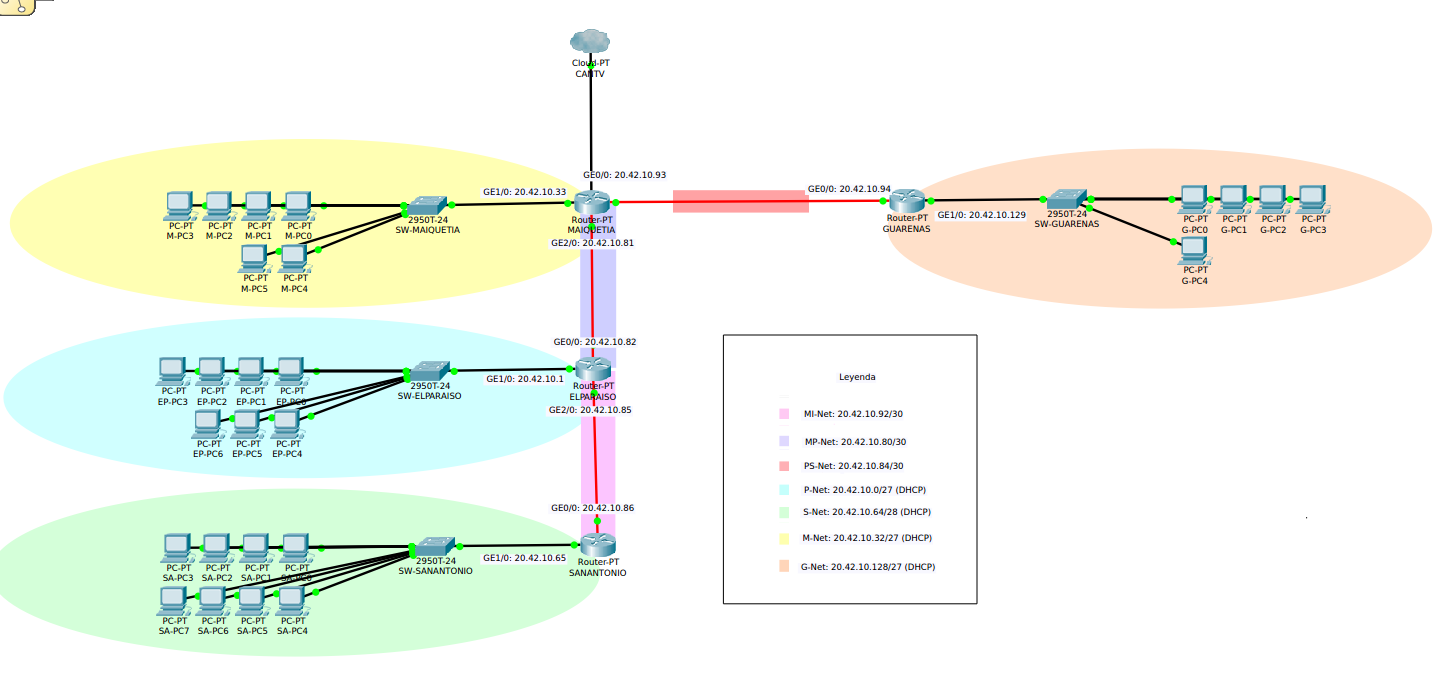
\includegraphics{ModeloAlternoCostosos.png}\\

\paragraph{Modelo 2}\label{modelo-2}

En este modelo, las redes de Guarenas y Maiquetía estan conectadas
mediante el ISP, mientras que Maiquetia establece conexión con El
Paraiso y San Antonio. Este modelo fué descartado debido a los costos
requeridos para conectar Maiquetía y San Antonio, teniendo como
alternativa inmediata el próximo modelo.

\paragraph{Modelo 3}\label{modelo-3}

En este modelo, las redes de Guarenas y Maiquetía estan conectadas
mediante el ISP, Maiquetía establece conexión con El Paraiso y este con
San Antonio. El enrutador de El Paraiso funciona como enlace entre
Maiquetía y San Antonio. Este modelo es el que se seleccionó debido a su
buena gestión de recursos y eficiencia en la red. Sin embargo, para que
pudiese funcionar, fue requerida la defición de enrutamiento explicada
más adelante.

\begin{figure}[htbp]
\centering
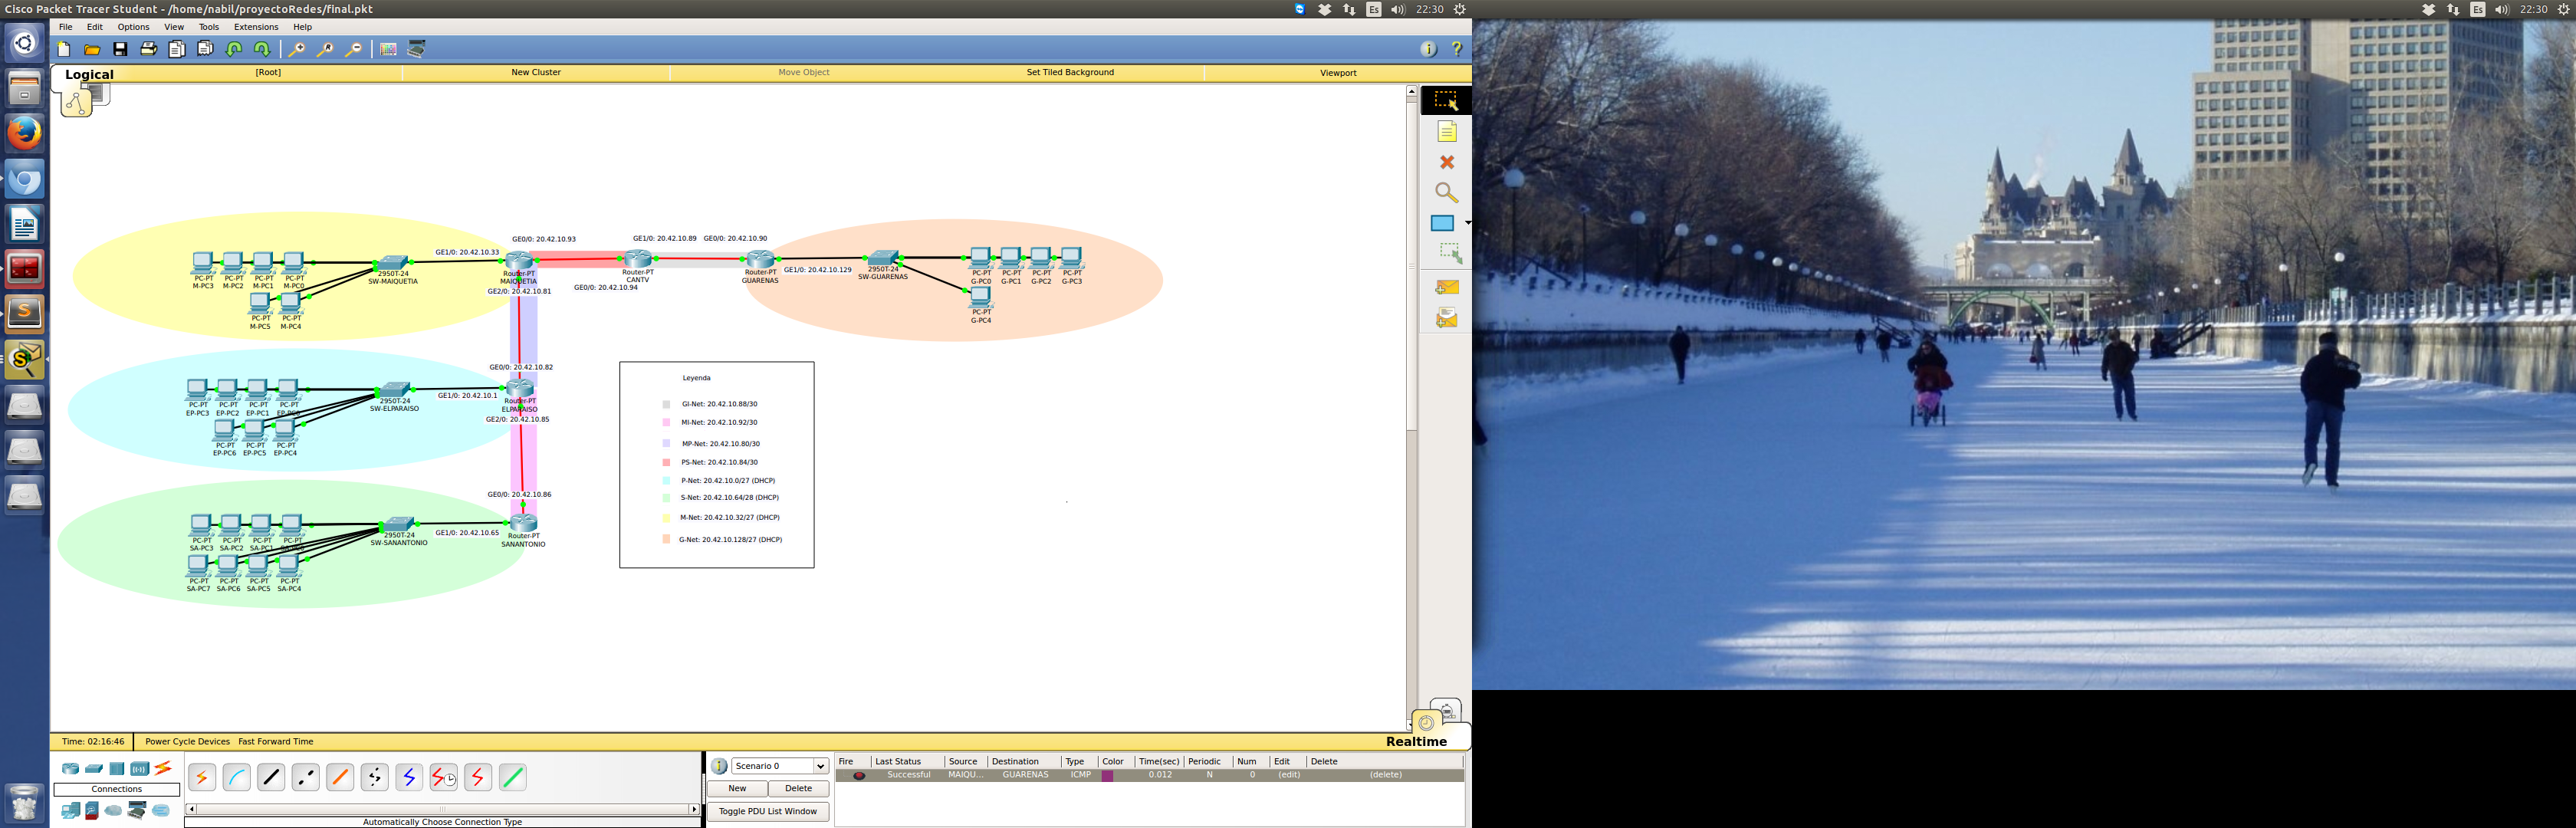
\includegraphics{ModeloFinal.png}
\caption{Modelo final}
\end{figure}

\newpage

\subsubsection{Descripción de la
topología}\label{descripciuxf3n-de-la-topologuxeda}

La topología escogida para implantar la red de Salud-Caracas está basada
en la topología de tipo Árbol. Como nodo raíz, se tiene al enrutador de
CANTV, y los hijos inmediatos a éste son el enrutador \emph{GUARENAS} y
el enrutador \emph{MAIQUETIA}. En el siguiente nivel se encuentran el
conmutador de Maiquetía, el enrutador \emph{ELPARAISO} y el conmutador
de Guarenas. Luego, se tienen a los hosts de Maiquetía, los host de
Guarenas, el conmutador de El Paraiso y el enrutador \emph{SANANTONIO}.
Luego de esto, están presente los host de El Paraiso y el conmutador de
San Antonio. En el último nivel, estan presentes los hosts de San
Antonio.

Para el caso particular de esta implantación, los ordenadores
representan las hojas del árbol ya que no tendrán hijos y los
conmutadores o los enrutadores representan el nodo padre de un árbol
subsiguiente.

\subsection{Esquema de
direccionamiento}\label{esquema-de-direccionamiento}

\subsubsection{Requisitos}\label{requisitos}

Tomando en cuenta que el crecimiento estimado se refiere a la cantidad
de host en la que puede incrementar la subred partiendo de la cantidad
presente, se tienen los siguientes requerimientos generales:

\begin{enumerate}
\def\labelenumi{\arabic{enumi}.}
\itemsep1pt\parskip0pt\parsep0pt
\item
  Una subred de 27 hosts para El paraiso (7 Actuales y 20 del
  crecimiento estimado).
\item
  Una subred de 8 hosts para San Antonio de los Altos.
\item
  Una subred de 15 hosts para Guarenas (5 Actuales y 10 del crecimiento
  estimado).
\item
  Una subred de 21 hosts para Maiquetía (6 Actuales y 15 del crecimiento
  estimado).
\end{enumerate}

\subsubsection{Analisís de requisitos:
totalización.}\label{analisuxeds-de-requisitos-totalizaciuxf3n.}

En cuanto al direccionamiento IP se refiere, se decidió comprar el rango
de direcciones IP del ISP CANTV asociadas a 20.42.10.0/24 ya que la red
es para una clínica de gran alcance y se disponen los medios para ello.
A su vez, si se desea a futuro construir otra sede de Salud-Caracas, se
dispondrían de direcciones IP para asignar a la nueva sede.

Estableciendo etiquetas para cada subred, se tiene:

P-net = El Paraiso. S-net = San Antonio de los Altos. G-net = Guarenas.
M-net = Maiquetía.

Inicialmente se poseen dos enrutadors con direcciones IP asignadas
mediante el ISP CANTV, cada uno con su respectiva subred.

\begin{longtable}[c]{@{}llll@{}}
\toprule\addlinespace
Subred & Nº Hosts & Crec. Estim. & Enrutadores
\\\addlinespace
\midrule\endhead
P-net & 7 & 20 & 1
\\\addlinespace
M-net & 6 & 15 & 1
\\\addlinespace
G-net & 5 & 10 & 1
\\\addlinespace
S-net & 8 & 0 & 1
\\\addlinespace
\bottomrule
\end{longtable}

Sin embargo, al requerir interconectar los enrutadors de Caracas (sin
incurrir en costos adicionales para cables al tomar a El Paraiso como
nodo central), es necesario crear 2 sub-redes nuevas, MP-net y PS-net, a
su vez son requeridas otras dos para las conexiones de Guarenas al ISP y
del ISP a Maiquetia.

Actualizando la tabla anterior de esta manera:\\\\

\begin{longtable}[c]{@{}llll@{}}
\toprule\addlinespace
Subred & Nº Hosts & Crec. Estim. & Enrutadores
\\\addlinespace
\midrule\endhead
P-net & 7 & 20 & 1
\\\addlinespace
M-net & 6 & 15 & 1
\\\addlinespace
G-net & 5 & 10 & 1
\\\addlinespace
S-net & 8 & 0 & 1
\\\addlinespace
MP-net & 2 & 0 & 0
\\\addlinespace
PS-net & 2 & 0 & 0
\\\addlinespace
GI-net & 2 & 0 & 0
\\\addlinespace
MI-net & 2 & 0 & 0
\\\addlinespace
\bottomrule
\end{longtable}

\begin{longtable}[c]{@{}llll@{}}
\toprule\addlinespace
\begin{minipage}[t]{0.17\columnwidth}\raggedright
TOTAL
\end{minipage} & \begin{minipage}[t]{0.17\columnwidth}\raggedright
34
\end{minipage} & \begin{minipage}[t]{0.17\columnwidth}\raggedright
45
\end{minipage} & \begin{minipage}[t]{0.17\columnwidth}\raggedright
4
\end{minipage}
\\\addlinespace
\bottomrule
\end{longtable}

A partir de la tabla anterior, se puede inferir la cantidad de host
necesarios para cada supra-red principal, siendo:

\begin{itemize}
\itemsep1pt\parskip0pt\parsep0pt
\item
  PMS-net = P-net, S-net, M-net, MP-net y PS-net.
\item
  G-net = G-net.
\end{itemize}

\begin{longtable}[c]{@{}lllllll@{}}
\toprule\addlinespace
Subred & Nº Hosts & Crec. Estim. & Enrutadores & Req. total & Máscara &
IP's Libres
\\\addlinespace
\midrule\endhead
PMS-net & 25 & 35 & 3 & 63 & /25 \footnote{Representación decimal
  255.255.255.128} & 63
\\\addlinespace
G-net & 5 & 10 & 1 & 16 & /27 \footnote{Representación decimal
  255.255.255.224} & 14
\\\addlinespace
\bottomrule
\end{longtable}

A pesar de que para la G-net se están desperdiciando 14 direcciones,
utilizar una máscara más pequeña implicaría aumentar los costos al tener
que utilizar otro enrutador con máscara 255.255.255.252 y los otros
instrumentos asociados (conmutadores, cables, interfaces de red). Como
se esta considerando la mejor opción costo-rendimiento, se dejará libre
ese rango de direcciones con el fin de evitar costos adicionales.
Análogamente para la PMS-net.

\newpage

\subsubsection{Analisís de requisitos: Información detallada de las
subredes.}\label{analisuxeds-de-requisitos-informaciuxf3n-detallada-de-las-subredes.}

Sin procesar las subredes en PMS-net, se tiene:

Luego se aplicó la técnica de LVSM para la distribución de direcciones
IP en estas subredes, debido a que existen diferencias notables en
cuanto a la cantidad de hosts requeridas por cada subred como para
realizar una distribución estática. Luego de aplicar esta técnica, se
obtuvo:

\begin{longtable}[c]{@{}llllll@{}}
\toprule\addlinespace
Subred & Máscara & Dir Subred & Broadcast & Rango & D. Libres
\\\addlinespace
\midrule\endhead
PMS-net & 255.255.255.128 & 20.42.10.0 & 20.42.10.127 & .1 -
.126\footnote{Todos rangos poseen el prefijo 20.42.10} & 63
\\\addlinespace
G-net & 255.255.255.224 & 20.42.10.128 & 20.42.10.159 & .129 - .159 & 14
\\\addlinespace
\bottomrule
\end{longtable}

Y las subredes de la PMS-net estan conformadas de esta manera:

\begin{longtable}[c]{@{}llllll@{}}
\toprule\addlinespace
Subred & Máscara & Dir Subred & Broadcast & Rango & D. Libres
\\\addlinespace
\midrule\endhead
P-net & 255.255.255.224 & 20.42.10.0 & 20.42.10.31 & .1 - .30\footnote{Todos
  rangos poseen el prefijo 20.42.10} & 2
\\\addlinespace
M-net & 255.255.255.224 & 20.42.10.32 & 20.42.10.63 & .33 - .62 & 8
\\\addlinespace
S-net & 255.255.255.240 & 20.42.10.64 & 20.42.10.79 & .65 - .78 & 5
\\\addlinespace
MP-net & 255.255.255.252 & 20.42.10.80 & 20.42.10.83 & .81 - .82 & 0
\\\addlinespace
PS-net & 255.255.255.252 & 20.42.10.84 & 20.42.10.87 & .85 - .86 & 0
\\\addlinespace
GI-net & 255.255.255.252 & 20.42.10.88 & 20.42.10.91 & .89 - .90 & 0
\\\addlinespace
MI-net & 255.255.255.252 & 20.42.10.92 & 20.42.10.95 & .93 - .94 & 0
\\\addlinespace
\bottomrule
\end{longtable}

\subsection{Enrutamiento}\label{enrutamiento}

\subsubsection{Descripción del
enrutamiento}\label{descripciuxf3n-del-enrutamiento}

Debido a la topología escogida, es necesario definir un enrutamiento
adecuado para poder interconectar adecuadamente las subredes entre sí y
que estas conozcan a que enrutador siguiente consultar.

A pesar de disponer de la opción de utilizar enrutamiento dinámico, se
decidió utilizar enrutamiento estático ya que la carga extra que
requiere el enrutamiento dinámico es innecesaria para la topología
escogida. Así, cada enrutador se encarga o bien de enviar el paquete a
un host de su subred o de enviarlo al siguiente enrutador que contenga
la tabla de enrutamiento de la subred a la que va dirigida el paquete
recibido o conozca a que enrutador reenviarlo.

Con el propósito de no afectar la funcionalidad del modelo lógico
planteado utilizando la herramienta \emph{Packet Tracer}, el router que
representa a CANTV posee un enrutamiento estático, sin embargo, para
efectos de su equivalencia en la topología en el mundo real, este
enrutamiento sería ofrecido y configurado por el ISP.

\subsubsection{Código implantado}\label{cuxf3digo-implantado}

Se utilizó el Control Line Interface de cada enrutador para configurar
el enrutamiento estático correspondiente.

\begin{verbatim}
SANANTONIO(config)#ip route 20.42.10.0 255.255.255.224 20.42.10.85
SANANTONIO(config)#ip route 20.42.10.32 255.255.255.224 20.42.10.85
SANANTONIO(config)#ip route 20.42.10.80 255.255.255.252 20.42.10.85
SANANTONIO(config)#ip route 20.42.10.92 255.255.255.252 20.42.10.85
SANANTONIO(config)#ip route 20.42.10.128 255.255.255.224 20.42.10.85
SANANTONIO(config)#ip route 20.42.10.88 255.255.255.252 20.42.10.85

---------------------------

ELPARAISO(config)#ip route 20.42.10.32 255.255.255.224 20.42.10.81
ELPARAISO(config)#ip route 20.42.10.88 255.255.255.252 20.42.10.81
ELPARAISO(config)#ip route 20.42.10.92 255.255.255.252 20.42.10.81
ELPARAISO(config)#ip route 20.42.10.128 255.255.255.224 20.42.10.81
ELPARAISO(config)#ip route 20.42.10.64 255.255.255.240 20.42.10.86

---------------------------

MAIQUETIA(config)#ip route 20.42.10.0 255.255.255.224 20.42.10.82
MAIQUETIA(config)#ip route 20.42.10.64 255.255.255.240 20.42.10.82
MAIQUETIA(config)#ip route 20.42.10.84 255.255.255.252 20.42.10.82
MAIQUETIA(config)#ip route 20.42.10.88 255.255.255.252 20.42.10.94
MAIQUETIA(config)#ip route 20.42.10.128 255.255.255.224 20.42.10.94

--------------------------

CANTV(config)#ip route 20.42.10.0 255.255.255.224 20.42.10.93
CANTV(config)#ip route 20.42.10.32 255.255.255.224 20.42.10.93
CANTV(config)#ip route 20.42.10.64 255.255.255.224 20.42.10.93
CANTV(config)#ip route 20.42.10.64 255.255.255.240 20.42.10.93
CANTV(config)#ip route 20.42.10.80 255.255.255.252 20.42.10.93
CANTV(config)#ip route 20.42.10.84 255.255.255.252 20.42.10.93


--------------------------

GUARENAS(config)#ip route 20.42.10.0 255.255.255.224 20.42.10.89
GUARENAS(config)#ip route 20.42.10.32 255.255.255.224 20.42.10.89
GUARENAS(config)#ip route 20.42.10.64 255.255.255.240 20.42.10.89
GUARENAS(config)#ip route 20.42.10.80 255.255.255.252 20.42.10.89
GUARENAS(config)#ip route 20.42.10.84 255.255.255.252 20.42.10.89
GUARENAS(config)#ip route 20.42.10.92 255.255.255.252 20.42.10.89
\end{verbatim}

\subsection{Direccionamiento IP}\label{direccionamiento-ip}

\subsubsection{Descripción del direccionamiento
IP}\label{descripciuxf3n-del-direccionamiento-ip}

Se utilizó DHCP ya que esto facilita la configuración en presencia de
subredes grandes o que poseen un crecimiento estimado considerable.
Adicionalmente a esto, en ninguna de las subredes diseñadas para
Salud-Caracas se ofrecen servicios fuera de los routers, por lo que no
es necesario establecer direcciones estáticas en estas.

Otra ventaja de esta decisión es el hecho de que representa un ahorro en
la configuración de la red en la que se disponga de este servidor DHCP
en el momento en el que se adquieran nuevos ordenadores y se conecten a
la red: ni estos, ni el servidor, requerirán alguna configuración
adicional a la proporcionada inicialmente. Adicionalmente, debido a las
fallas en el servicio eléctrico del país los ordenadores están propensos
al deterioro, de esta forma su reemplazo ser'ia mucho más simple, de
forma análoga al caso anteriormente expuesto.

\subsubsection{Código implantado}\label{cuxf3digo-implantado-1}

Se utilizó el Control Line Interface de cada enrutador para configurar
el servidor DHCP asociado a la subred que cada enrutador esté encargado
de interconectar.

\begin{verbatim}
GUARENAS(config)#ip dhcp pool GNET
GUARENAS(dhcp-config)#network 20.42.10.128 255.255.255.224
GUARENAS(dhcp-config)#default-enrutador 20.42.10.129
GUARENAS(dhcp-config)#dns-server 8.8.8.8
GUARENAS(dhcp-config)#exit
GUARENAS(config)#do wr

---------------------------

MAIQUETIA(config-if)#ip dhcp pool MNET
MAIQUETIA(dhcp-config)#network 20.42.10.32 255.255.255.224
MAIQUETIA(dhcp-config)#default-enrutador 20.42.10.33
MAIQUETIA(dhcp-config)#dns-server 8.8.8.8
MAIQUETIA(dhcp-config)#exit
MAIQUETIA(config)#do wr

---------------------------

ELPARAISO(config-if)#ip dhcp pool PNET
ELPARAISO(dhcp-config)#network 20.42.10.0 255.255.255.224
ELPARAISO(dhcp-config)#dns-server 8.8.8.8
ELPARAISO(dhcp-config)#default-enrutador 20.42.10.1
ELPARAISO(dhcp-config)#exit
ELPARAISO(config)#do wr

---------------------------

SANANTONIO(config-if)#ip dhcp pool SNET
SANANTONIO(dhcp-config)#default-enrutador 20.42.10.65
SANANTONIO(dhcp-config)#dns-server 8.8.8.8
SANANTONIO(dhcp-config)#network 20.42.10.64 255.255.255.240
SANANTONIO(dhcp-config)#exit
SANANTONIO(config)#do wr
\end{verbatim}

\subsection{Dispositivos requeridos}\label{dispositivos-requeridos}

\subsubsection{Requerimientos}\label{requerimientos}

Los dispotivos utilizados en nuestra implementación incluyen:

\begin{itemize}
\itemsep1pt\parskip0pt\parsep0pt
\item
  4 enrutadores todos con al menos un conector de ethernet
  (preferiblemente gigagit)

  \begin{itemize}
  \itemsep1pt\parskip0pt\parsep0pt
  \item
    2 con 2 conectores de fibra óptica
  \item
    2 con 1 conector de fibra óptica
  \end{itemize}
\item
  5 conmutadores o \emph{switches} con las siguientes especificaciones

  \begin{itemize}
  \itemsep1pt\parskip0pt\parsep0pt
  \item
    1 de 16 puertos para la subred de Guatire
  \item
    1 de 24 puertos para la subred de El Paraiso (soporte para 22 hosts)
  \item
    1 de 6 puertos como auxiliar para la subred anterior (soporte para
    los 5 hosts faltantes)
  \item
    1 de 24 puertos para la subred Maiquetía
  \item
    1 de 16 puetos para la subred de San Antonio
  \end{itemize}
\item
  Bobina de cable de par trenzado categoría 5 (metraje dependiente de
  las distancias entre hosts)
\item
  Inicialmente 52 Conectores RJ45 categoría 5 , 90 adicionales para
  cubrir el crecimiento de las red.

  \begin{itemize}
  \itemsep1pt\parskip0pt\parsep0pt
  \item
    52 para los hosts iniciales
  \item
    90 para los hosts del crecimiento estimado
  \end{itemize}
\item
  Bobina de cable de par trenzado categoría 6
\item
  10 conectores RJ45 categoría 6 para las conexiones entre conmutadores
  y enrutadores
\item
  Bobina de fibra óptica 2 hilos multimodo (metraje dependiente de las
  conexiones existentes que el ISP provea)
\item
  6 conectores de fibra óptica multimodo de 2 hilos, \emph{pigtail upc}
\end{itemize}

Cada \emph{switch} debería tener al menos un puerto gigabit para
conectar con su respectivo \emph{router}.

El conmutador de El Paraiso que conecta un conjuntos de hosts, el router
y segundo conmutador pequeño (de 6 puertos) requiere de 2 puertos
gigabit.

La cantidad de metros de cable entre cada host y su conmutador más
cercano es variable, además depende del tamaño de cada centro médico en
el que se está integrando la red. Suponiendo distancias de 3 ó 10 metros
como media se requerirían al menos 78 metros de cable, y a lo más 260
como distancias iniciales. Luego del crecimiento esperado se utilizaría
entre 213 y 710 metros de cable categoría 5. El plan incial de red
requiere de 52 conectores RJ45 y al final del crecimiento esperado se
habrán usado 142 para ensamblar los cables de red.

Para las instalaciones de cableado entre routers (fibra óptica) no se
conoce con exactitud la cantidad de conexiones entre preexistentes que
provee el ISP de CANTV, ya que podría o no existir las conexiones entre
una central de CANTV y un lugar cercano a los routers de Maiquetía y
Guarenas, por lo que presentamos dos planes de requerimientos.

Como plan básico, para ambos planes se debe colocar cableado entre San
Antonio y El Paraiso, y entre éste y Maiquetía, lo que representa (de
acuerdo a la sección de nuestro análisis preliminar) una cantidad total
de 58.3 km (suma de ambos segmentos). Dependiendo de las conexiones de
CANTV se podría requererir entre 20 metros para conectar los centros de
Salud-Caracas en Maiquetía y Guarenas al \emph{router} más cercano del
ISP, o utilizar, en el peor escenario posible 65 km de fibra óptica para
conectar ambas instalaciones pasando por el router de CANTV. CANTV
debería proveer de esta última conexión, por lo que el último plan de
requerimiento no será tomado en cuenta. De esta manera se utilizarán
unicamente 58.5 kilómetros de la fibra óptica ya especificada.

Cada cable de fibra óptica será ensamblado con 2 conectores pigtail.

Por último para realizar las conexiones entre los enrutadores de cada
ciudad y su conmutador asociado y entre conmutadores (en El Paraíso) y
suponiendo distancias de 5 metros entre cada uno de estos, se requerirán
25 metros de cable categoría 6, los cuales serán ensamblados con
conectores RJ45 cat6.

\newpage

\subsubsection{Costos}\label{costos}

Realizando los cálculos con a SIMADI del 4/6/2016 (549 Bs por \$) para
el cable de fibra óptica y los routes.

Los costos aproximados obtenidos los portales de compras por internet
mercadolibre y alibaba (a tasa SIMADI) arrojan la siguiente tabla de
presupuesto:

\begin{longtable}[c]{@{}lccc@{}}
\toprule\addlinespace
Item & Costo (Bs) & Cantidad & Total (Bs)
\\\addlinespace
\midrule\endhead
Switch TP-link 16 puertos gigabit & 149.000 & 2 & 29.9998
\\\addlinespace
Switch cisco 24 con 2 puertos gigabit & 219.000 & 2 & 438.000
\\\addlinespace
Switch 8 puertos gigabit & 32.900 & 1 & 32.900
\\\addlinespace
Enrutador, con puertos de fibra optica y gigabit & 384.300 & 4 &
1.537.200
\\\addlinespace
\bottomrule
\end{longtable}

\begin{longtable}[c]{@{}ll@{}}
\toprule\addlinespace
\begin{minipage}[t]{0.18\columnwidth}\raggedright
TOTAL
\end{minipage} & \begin{minipage}[t]{0.21\columnwidth}\raggedright
2.308.098
\end{minipage}
\\\addlinespace
\bottomrule
\end{longtable}

\begin{longtable}[c]{@{}lccc@{}}
\toprule\addlinespace
Item & Costo (Bs) & Cantidad & Total (Bs)
\\\addlinespace
\midrule\endhead
Pigtails & 5.990 & 6 & 35.940
\\\addlinespace
RJ45 cat6 blindado & 650 & 10 & 6.500
\\\addlinespace
RJ45 cat5 (100 unidades) & 3.250 & 1 & 3.250
\\\addlinespace
Bobina cat5E 305 metros & 36.990 & 1 & 36.990
\\\addlinespace
Bobina cat6 por metro & 600 & 25 & 15.990
\\\addlinespace
Fibra óptica por km & 54.900 & 58.5 & 3.211.650
\\\addlinespace
\bottomrule
\end{longtable}

Sin contar los gatos por fibra óptica el valor para las conexiones será
de Bs. 98.670, incluyendola obtendremos el siguiente monto:

\begin{longtable}[c]{@{}ll@{}}
\toprule\addlinespace
\begin{minipage}[t]{0.18\columnwidth}\raggedright
TOTAL
\end{minipage} & \begin{minipage}[t]{0.21\columnwidth}\raggedright
3.310.320
\end{minipage}
\\\addlinespace
\bottomrule
\end{longtable}

El total de conectividad y dispotivos de conexión será de Bs 5.618.418

La compra de la bobina de categoría 5 de 305 metros cubrirá el
requerimiento inicial para los hosts y (potencialmente) cubrirá la
demanda de los hosts nuevos (todo depende de las distancias explicadas
en la sección anterior).

El costo del conjunto de direcciones IP públicas utilizadas no está
contemplado en el presupuesto, ya que CANTV no ofrece precios en su
portal.

\subsection{Explicaciones adicionales}\label{explicaciones-adicionales}

\begin{itemize}
\itemsep1pt\parskip0pt\parsep0pt
\item
  Se descartó el uso de de redes inalámbricas para los centros médicos
  ya que esto implicaría el uso de \emph{access point} con alcance
  metropolitano y tarjetas inalámbricas para cada hosts, lo cual
  implicaría un gran aumento en el costo total de la implementación de
  este proyecto.
\item
  Se utilizaron cable categoría 6 entre conmutadores y enrutadores para
  mejorar las velocidades de conexión y ancho de banda, sin aumentar
  drásticamente los costos al hacer uso de este cable para cada uno de
  los hosts, además esto implicaría instalar un gran número de tarjetas
  de red \emph{gigabit} en vez de utilizar las \emph{fast-ethernet} que
  usualmente incluyen las computadoras.
\item
  Se decidió realizar la importación de fibra óptica ya que reducía los
  costros en gran medida. Mientras que la importación de los routers fue
  motivada por la ausencia de este producto en el mercado nacional.
\item
  No se incluyó el costo de la instalación de los cables de fibra óptico
  y sus canales.
\item
  A pesar de existir otros tipos topológicos como el basado en malla, el
  mixto o el anillo, se optó por el presente debido a sus bajos costos
  en comparación. Colocar una conexion entre Maiquetía y San Antonio o
  San Antonio y Guarenas,realizando la redistribución ip requerida y el
  enrutamiento adecuado, se ofrecería una mejor tolerancia a fallos ya
  que existe mayor interconexión entre las sburedes, pero los costos
  aumentaría en gran nivel debido a la distancias físicas entre cada
  nodo. Se sacrifica la recuperación de errores para economizar los
  costos, sin embargo, la topología actual admite futuras modificaciones
  según sea requerido.
\end{itemize}

\section{Referencias}\label{referencias}

\subsection{Mercadolibre}\label{mercadolibre}

Portal de ventas en línea en Venezuela

\begin{itemize}
\itemsep1pt\parskip0pt\parsep0pt
\item
  Swith Tp-Link de 16 puertos gigabit

  \begin{itemize}
  \itemsep1pt\parskip0pt\parsep0pt
  \item
    http://articulo.mercadolibre.com.ve/MLV-463531660-switch-gigabit-de-16-puertos-tp-link-tl-sg1016-\_JM
  \end{itemize}
\item
  Switch cisco de 24 puertos (2 gigabit)

  \begin{itemize}
  \itemsep1pt\parskip0pt\parsep0pt
  \item
    http://articulo.mercadolibre.com.ve/MLV-462458481-switch-cisco-sf200-24-24-puertos-10100-2-puertos-gigabit-\_JM
  \end{itemize}
\item
  Switch Advantek de 8 puertos gigabit

  \begin{itemize}
  \itemsep1pt\parskip0pt\parsep0pt
  \item
    http://articulo.mercadolibre.com.ve/MLV-465748796-switch-gigabit-advantek-8-puertos-101001000-netpro-serie-\_JM
  \end{itemize}
\item
  Conectores de fibra óptica

  \begin{itemize}
  \itemsep1pt\parskip0pt\parsep0pt
  \item
    http://articulo.mercadolibre.com.ve/MLV-465234972-pigtails-fibra-optica-multimodo-sc-upc-azul-\_JM
  \end{itemize}
\item
  Conectores RJ45 categoría 6

  \begin{itemize}
  \itemsep1pt\parskip0pt\parsep0pt
  \item
    http://articulo.mercadolibre.com.ve/MLV-465127459-conector-rj45-cat6-blindado-lanpro-gigabit-red-internet-\_JM
  \end{itemize}
\item
  Conectores RJ45 categoría 5

  \begin{itemize}
  \itemsep1pt\parskip0pt\parsep0pt
  \item
    http://articulo.mercadolibre.com.ve/MLV-465432656-conector-rj-45-cat-5e-paquete-de-100-unidades-\_JM
  \end{itemize}
\item
  Bobina de cable categoría 5 (305 metros)

  \begin{itemize}
  \itemsep1pt\parskip0pt\parsep0pt
  \item
    http://articulo.mercadolibre.com.ve/MLV-465913392-bobina-cable-utp-cat5e-305-mts-rj45-cctv-redes-seguridad-lan-\_JM
  \end{itemize}
\item
  Cable categoría 6 por metro

  \begin{itemize}
  \itemsep1pt\parskip0pt\parsep0pt
  \item
    http://articulo.mercadolibre.com.ve/MLV-459248117-cable-utp-categoria-6-100-cobre-por-metro-\_JM
  \end{itemize}
\end{itemize}

\section{Amazon}\label{amazon}

Portal de ventas norteamericano

\begin{itemize}
\itemsep1pt\parskip0pt\parsep0pt
\item
  Cisco CISCO2911/K9 2911 2900 Series Integrated Services Router

  \begin{itemize}
  \itemsep1pt\parskip0pt\parsep0pt
  \item
    http://www.amazon.com/gp/offer-listing/B002ZCUCLS/ref=olp\_f\_refurbished?ie=UTF8\&f\_refurbished=true\&f\_used=true\&f\_usedAcceptable=true\&f\_usedGood=true\&f\_usedLikeNew=true\&f\_usedVeryGood=true\&qid=1465217516\&sr=8-1
  \end{itemize}
\end{itemize}

\subsection{Alibaba}\label{alibaba}

Portal de ventas al mayor por internet de proveedores ubicados en Asia

\begin{itemize}
\itemsep1pt\parskip0pt\parsep0pt
\item
  Cable de fibra óptica por kilómetro

  \begin{itemize}
  \itemsep1pt\parskip0pt\parsep0pt
  \item
    http://www.alibaba.com/product-detail/Outdoor-direct-buried-amored-fiber-optic\_213229352.html?spm=a2700.7724838.0.0.CzmEbD\&s=p
  \end{itemize}
\end{itemize}

\subsection{CANTV}\label{cantv}

\begin{itemize}
\itemsep1pt\parskip0pt\parsep0pt
\item
  Planes y servicios

  \begin{itemize}
  \itemsep1pt\parskip0pt\parsep0pt
  \item
    http://www.cantv.com.ve/seccion.asp?pid=1\&sid=607
  \end{itemize}
\end{itemize}

\subsection{Referencias teóricas}\label{referencias-teuxf3ricas}

\begin{itemize}
\itemsep1pt\parskip0pt\parsep0pt
\item
  Configuración de VPN

  \begin{itemize}
  \itemsep1pt\parskip0pt\parsep0pt
  \item
    http://ecovi.uagro.mx/ccna4/course/files/7.1.2.4\%20Packet\%20Tracer\%20-\%20Configuring\%20VPNs\%20\%28Optional\%29\%20Instructions.pdf
  \item
    http://showipprotocols.blogspot.com/2015/05/site-to-site-ipsec-vpn-configuration.html
  \item
    http://securitywing.com/cisco-vpn-configuration/
  \end{itemize}
\item
  Referencia de packet-tracer

  \begin{itemize}
  \itemsep1pt\parskip0pt\parsep0pt
  \item
    http://www.cisco.com/c/en/us/td/docs/security/asa/asa80/configuration/guide/conf\_gd/site2sit.pdf
  \end{itemize}
\item
  Configuración de DHCP

  \begin{itemize}
  \itemsep1pt\parskip0pt\parsep0pt
  \item
    https://www.youtube.com/watch?v=yudNmI4p1dU
  \item
    https://fpomicro.wordpress.com/2011/11/29/configurar-dhcp-en-router-cisco-packet-tracer-5-3/
  \item
    http://www.mws.cz/network/packet-tracer/router-dhcp/
  \end{itemize}
\end{itemize}

\end{document}
